\documentclass[a4paper, 10pt, danish, final]{article}
\usepackage{bonde}

\def\mytitle{Dataanalyse 2010}
\def\mysubtitle{Aflevering af ugeopgave 2}
\def\myauthor{Ulrik Bonde}
\def\mymail{\mailto{bonde@diku.dk}}
\def\mydate{\today}
\def\repository{\url{http://github.com/bonde/dataanalyse}}

\title{\mytitle}
\subtitle{\mysubtitle}

\author{\myauthor{} - \mymail}
\date{\mydate}

\hypersetup{
colorlinks,%
citecolor=black,%
filecolor=black,%
linkcolor=black,%
urlcolor=black,%
bookmarksopen=false,
pdftitle={\mytitle{} - \mysubtitle},
pdfauthor={\myauthor}
}

\begin{document}
\maketitle

\subsection*{Spørgsmål 1}
Jeg vil i denne opgave bruge et meget simpelt billede til at illustrere
den to-dimensionelle Fouriertransformation og effekten af ideel
filtrering af billeder. Billedet er vist i figur \ref{square} og er en
hvid firkant på en sort baggrund.

\begin{figure}[!h]
    \centering
    
\includegraphics[angle=0,width=0.45\textwidth]{images/square}
    \caption[]{Billedet som vi vil arbejde med. Motivet et simpelt og
    der er skarpe kontraster.}
    \label{square}
\end{figure}

Vi vil nu gerne finde billedets Fouriertransformation og vise det med og
uden translation af Origo til billedets midte. Fremgangsmåden er vist i
kodeboks \ref{fft_matlab} og de resulterende billeder er vist i figur
\ref{ffts}. I begge fremstillinger ses et tydeligt mønster, men først
når Origo translateres til midten bliver selve $sinc$-funktionen
åbenlys.

\begin{lstlisting}[caption={Fouriertransformation i MATLAB},
    captionpos=b, label={fft_matlab}, float=t, numbers=none]
% Read and show the original image
[I, cmap] = imread('../images/square.tiff', 'tiff');
figure; imshow(I, cmap);

% Show Fourier transform without shift
figure; imshow(log(abs(fft2(I))), cmap);

% Show Fourier transform with shift
figure; imshow(log(abs(fftshift(fft2(I)))), cmap);
\end{lstlisting}

\begin{figure}[!h]
    \centering
    \subfloat[Styrkespektret uden translation af Origo]{\label{fft_noshift}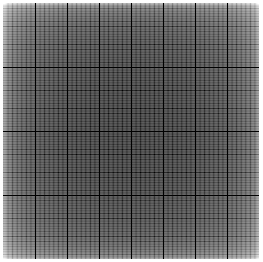
\includegraphics[angle=0,width=0.45\textwidth]{images/fft_noshift}\hspace{1em}}
    \subfloat[Styrkespektret med translation af Origo til
    billedecenteret]{\label{fft_shift}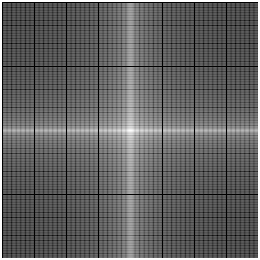
\includegraphics[angle=0,width=0.45\textwidth]{images/fft_shift}}
    \caption[]{To forskellige visninger af den samme
    Fouriertransformation. Billedet til venstre viser det egentlige
    output fra metoden \texttt{fft2} i MATLAB. Billedet til højre er
    blevet justeret således at vi har Origo i billedets midte.
    Billederne er lavet som vist i kodeboks \ref{fft_matlab}.}
    \label{ffts}
\end{figure}

Vi ønsker nu at filtrere billedet med et ideelt lav-pas-filter. Dette er
ligetil at gøre i frekvensdomænet, da vi blot kan skære de uønskede
frekvenser væk. Til filtrering er der vedlagt to MATLAB programmer.
\texttt{DAIdealFilter} opretter og returner det ideelle filter. Filteret
er defineret i frekvensdomænet og er blot en hvid cirkel som angiver
hvilke frekvenser vi lader passere.

Vi kan folde billedet og filteret i steddomænet, ved at lave punktvis
multiplikation i frekvensdomænet. \texttt{DAFilterF} gør dette lettere.
Den tager et billede og et frekvensfilter. Herefter Fouriertransformeres
billedet, mens filterets Origo translateres til øverste højere hjørne.
Nu udføres den punktvise multiplikation og vi kan returnere den inverse
Fouriertransformation. Billedet er nu blevet filtreret med det givne
filter.

I figur \ref{ideal_filter} er det vist og forklaret hvodan filtrering
med idealfilteret påvirker billedet.

\begin{figure}[!h]
    \centering
    \subfloat[Filter med $D_0 = 64$.]{\label{ideal_filter_64}
\includegraphics[angle=0,width=0.30\textwidth]{images/ideal_filter_64}}\hspace{1em}
    \subfloat[Filtreret frekvensdomæne]{\label{ideal_fft_64}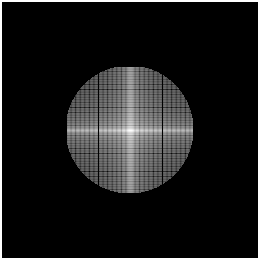
\includegraphics[angle=0,width=0.30\textwidth]{images/ideal_fft_64}}\hspace{1em}
    \subfloat[Filtreret billede]{\label{ideal_64}
\includegraphics[angle=0,width=0.30\textwidth]{images/ideal_64}}\\
    \subfloat[Filter med $D_0 = 32$.]{\label{ideal_filter_32}
\includegraphics[angle=0,width=0.30\textwidth]{images/ideal_filter_32}}\hspace{1em}
    \subfloat[Filtreret frekvensdomæne]{\label{ideal_fft_32}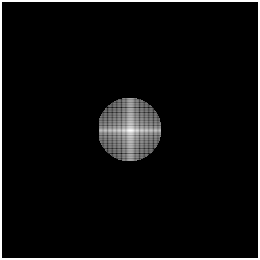
\includegraphics[angle=0,width=0.30\textwidth]{images/ideal_fft_32}}\hspace{1em}
    \subfloat[Filtreret billede]{\label{ideal_32}
\includegraphics[angle=0,width=0.30\textwidth]{images/ideal_32}}\\
    \subfloat[Filter med $D_0 = 16$.]{\label{ideal_filter_16}
\includegraphics[angle=0,width=0.30\textwidth]{images/ideal_filter_16}}\hspace{1em}
    \subfloat[Filtreret frekvensdomæne]{\label{ideal_fft_16}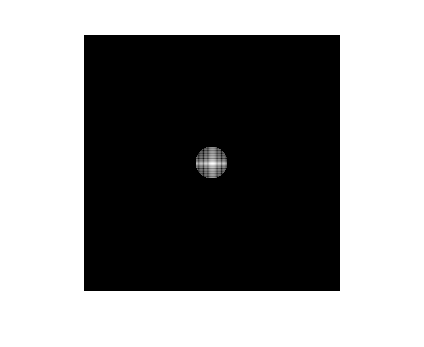
\includegraphics[angle=0,width=0.30\textwidth]{images/ideal_fft_16}}\hspace{1em}
    \subfloat[Filtreret billede]{\label{ideal_16}
\includegraphics[angle=0,width=0.30\textwidth]{images/ideal_16}}
    \caption[]{Tre forskellige filtreringer med idealfilteret med
    $D_0$ sat til hhv. 64, 32 og 16. Ved første filter ses det allerede
    at de skarpe kontraster udlignes ved brug af idealfilteret. Kanterne
    på firkanten bliver slørede og der ses ring-effekt. Dette
    intensiveres når $D_0$ bliver mindre, dvs. vi skærer flere høje
    frekvenser væk. Det ses at meget at billedeinformationen ligger i de
    lave frekvenser, da vi ved en lille værdi af $D_0$ stadig har en god
    fornemmelse af hvad billedet forestiller. Til at illustrere dette
    kunne man godt have brugt et andet billede.}
    \label{ideal_filter}
\end{figure}
\clearpage

\subsection*{Spørgsmål 2}
Vi er givet temperaturmålinger for hver time i 2009. Temperaturene er
vist i plottet i figur \ref{temp}.

\begin{figure}[!h]
    \centering
    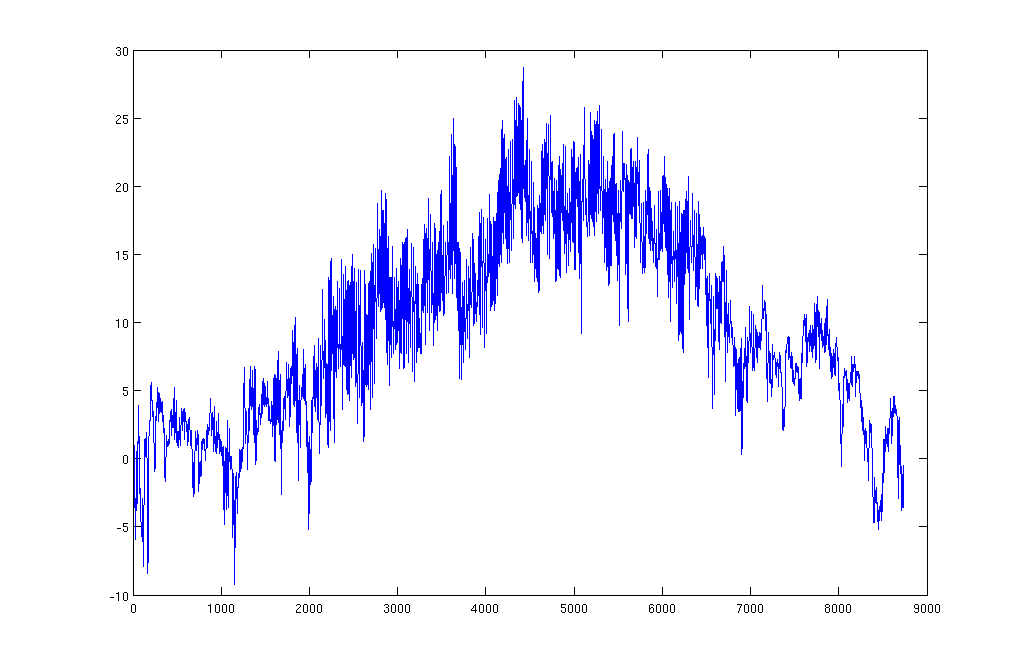
\includegraphics[angle=0,width=0.80\textwidth]{images/temp}
    \caption[]{Data fra filen \texttt{temp.mat}.}
    \label{temp}
\end{figure}

Fra plottet i figur \ref{temp} er det svært at sige noget om hvorvidt
signalet har periodiske strukturer, men man må antage at der vil være en
vis struktur mht. svingningen mellem dag- og nattetemperaturen. Det er
derfor interessant at kigge på det Fouriertransformerede signal som er
vist i figur \ref{ftemp}. I frekvensdomænet kan vi finde op til flere
symmetriske udslag som antyder periodiske strukturer i signalet.

\begin{figure}[!h]
    \centering
    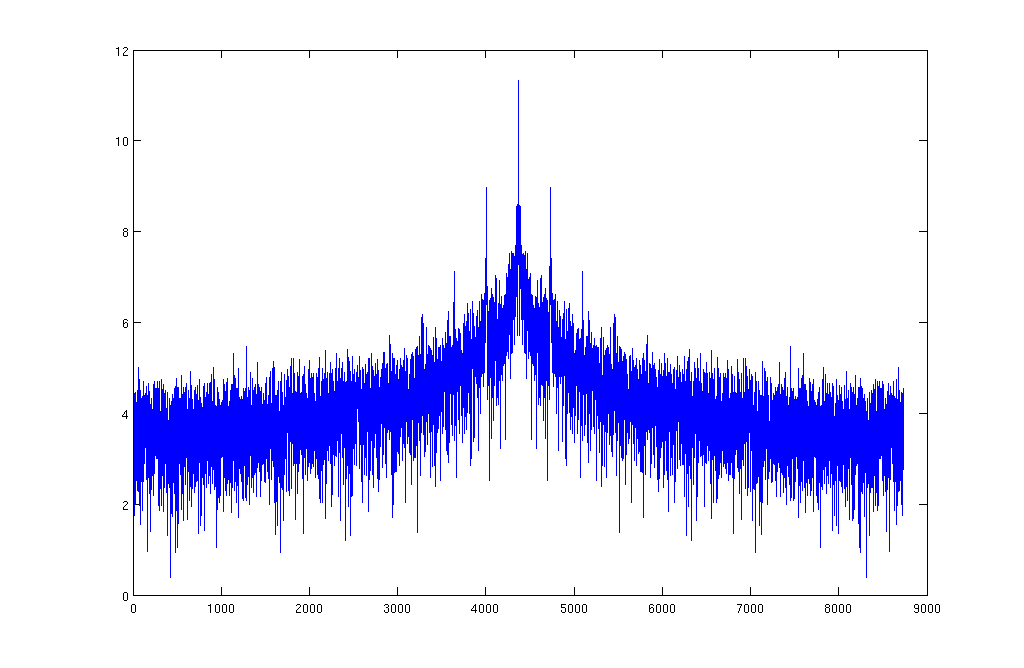
\includegraphics[angle=0,width=0.80\textwidth]{images/ftemp}
    \caption[]{Fouriertransformationen af temperaturmålinger. Der ses op
    til flere symmetriske maxima som antyder periodiske strukturer i
    signalet. Tydeligst er de to omkring Origo.}
    \label{ftemp}
\end{figure}

Vedlagt i bilag findes programmet \texttt{TempFilter} som giver mulighed
for at manipulere signalets frekvensdomæne. Ved at eksekvere kommandoen
\texttt{TempFilter(true)} kan man interaktivt klikke på de steder hvor
man ønsker at sætte signalet til 0. På denne måde kan man forsøge at
eliminere periodiske strukturer.

I praksis går det dog ikke så godt. At finde netop den frekvens som
udgør svingingen mellem nat- dagtemperatur er ikke lykkedes. I figur
\ref{temp_cut} er blot et af de utallige forsøg på at finde denne
frekvens vist.

Programmet kan også kaldes med argumentet \texttt{false} hvilket ikke
giver interaktiv filtrering. Derimod smides et ideelt lav-pas-filter
over signalet. Vi kommer nu tættere på at eliminere forskellen mellem
dag og nat. Resultatet er vist og videre kommenteret i figur
\ref{temp_low}.

Endeligt kan man ved en snedig udkommentering i linie 31 folde signalet
med en Gaussisk kerne. Dette er vist i figur \ref{temp_gauss}.
Umiddelbart giver denne filtrering af signalet det bedste resultat,
selvom de andre sikkert kan forbedres til en vis grad ved at justere
lidt på parametre og filtreringsområde.

\begin{figure}[!h]
    \centering
    \subfloat[Signal over en
    uge]{\label{temp_cut_1week}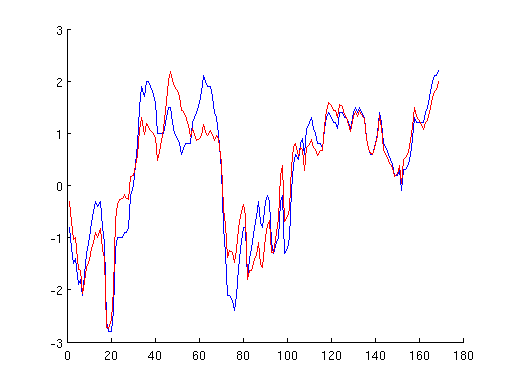
\includegraphics[angle=0,width=0.45\textwidth]{images/temp_cut_1week}}\hspace{1em}
    \subfloat[Signal over 4
    uger]{\label{temp_cut_4week}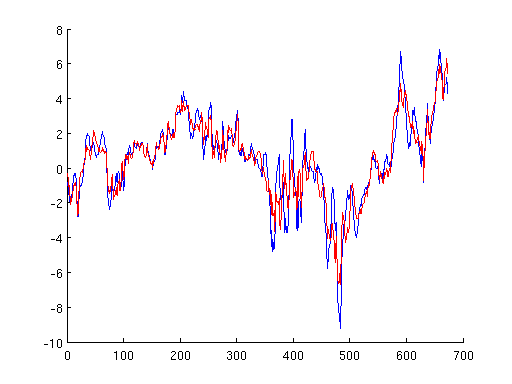
\includegraphics[angle=0,width=0.45\textwidth]{images/temp_cut_4week}}\\
    \subfloat[Modificeret
    frekvensdomæne]{\label{ftemp_cut}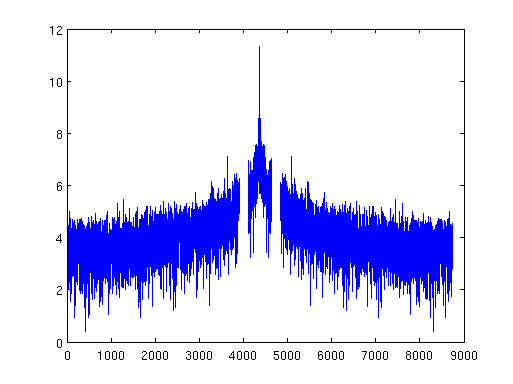
\includegraphics[angle=0,width=0.45\textwidth]{images/ftemp_cut}}
    \caption[]{De to maxima omkring Origo er skåret ud. Den blå kurve
    viser det originale signal, mens den røde er det filtrerede signal.
    Modifikationen i frekvensdomænet har kun ringe effekt på signalet og
    der er ingen antydning om at denne frekvens skulle være udsvinget
    mellem nat og dag.}
    \label{temp_cut}
\end{figure}

\begin{figure}[!h]
    \centering
    \subfloat[Signal over en
    uge]{\label{temp_low_1week}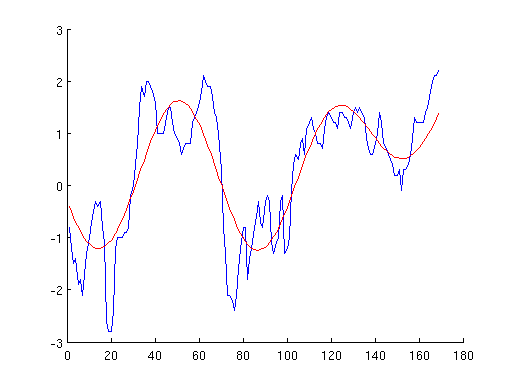
\includegraphics[angle=0,width=0.45\textwidth]{images/temp_low_1week}}\hspace{1em}
    \subfloat[Signal over 4
    uger]{\label{temp_low_4week}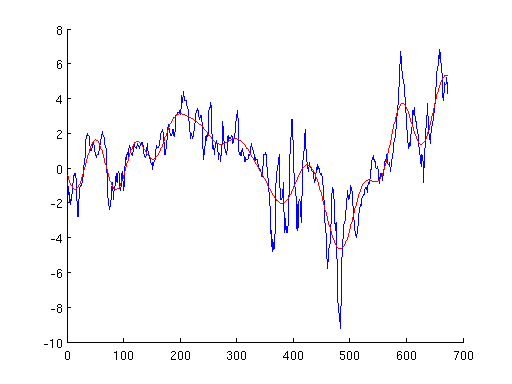
\includegraphics[angle=0,width=0.45\textwidth]{images/temp_low_4week}}\\
    \subfloat[Modificeret
    frekvensdomæne]{\label{ftemp_low}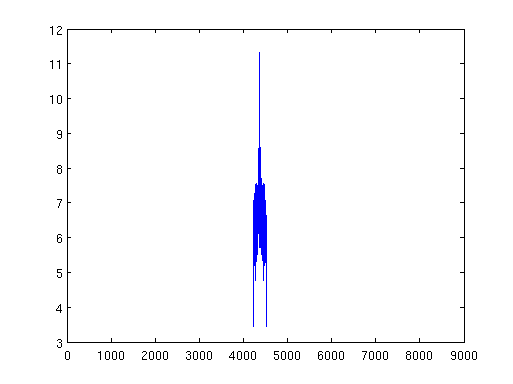
\includegraphics[angle=0,width=0.45\textwidth]{images/ftemp_low}}
    \caption[]{Meget groft idealt lav-pas-filter (med $D_0 = 150$).
    Selvom filteret er groft virker det nu meget godt. Der fjernes dog
    lidt for meget information og man kan i den grad sige at forskellen
    mellem nat og dag er blevet fjernet. Dette er et godt eksempel på
    hvor meget information der faktisk ligger i de lave frekvenser. Man
    skal dog være påpasselig med at bruge dette resultat på grund af
    idealfilteret og dets bieffekter (som vist i del 1).}
    \label{temp_low}
\end{figure}

\begin{figure}[!h]
    \centering
    \subfloat[Signal over en
    uge]{\label{temp_gauss_1week}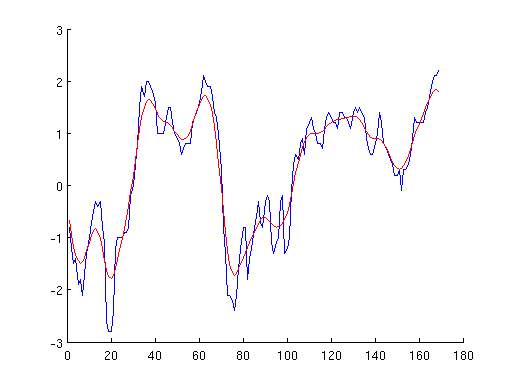
\includegraphics[angle=0,width=0.45\textwidth]{images/temp_gauss_1week}}\hspace{1em}
    \subfloat[Signal over 4
    uger]{\label{temp_gauss_4week}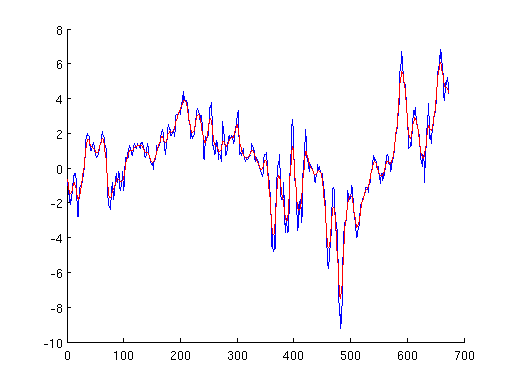
\includegraphics[angle=0,width=0.45\textwidth]{images/temp_gauss_4week}}\\
    \subfloat[Modificeret
    frekvensdomæne]{\label{ftemp_gauss}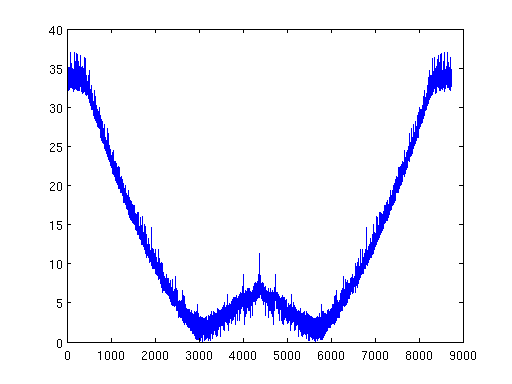
\includegraphics[angle=0,width=0.45\textwidth]{images/ftemp_gauss}}
    \caption[]{Signal foldet med en Gaussisk kerne med $\sigma = 3$. Det
    ses at signalet nu nærmer sig noget vi faktisk er interesseret i. De
    mindre udsving mellen nat og dag er blevet jævnet ud, men vi holder
    os overordnet set til kurven.}
    \label{temp_gauss}
\end{figure}

\clearpage

%%%%%%%%%%%%%%%%%%%%%%%%%%%%%%%%%%%%%%%%%%%%%%%%%%%%%%%%%%%%%%%%%%%%
% Formal stuff

%\bibliographystyle{abbrvnat}
%\bibliography{bibliography}
%\addcontentsline{toc}{chapter}{Litteratur}

\appendix
\lstset{language=Matlab, basicstyle=\scriptsize,
    showstringspaces=false, numbers=left, stepnumber=1,
    numberstyle=\tiny, frame=none}
\section{Kildekode}
Kildekoden er tilgængelig i mit git-repository på \repository{}. Bemærk
at prefikset \texttt{DA} står for ``DataAnalyse'' og blot er til for at
undgå eventuelle sammenstød med indbyggede funktioner i MATLAB.

\subsection{DAIdealFilter.m}
\lstinputlisting{../src/DAIdealFilter.m}

\subsection{DAFilterF.m}
\lstinputlisting{../src/DAFilterF.m}

\subsection{TempFilter.m}
\lstinputlisting{../src/TempFilter.m}

\end{document}

% vim: set tw=72 spell spelllang=da:
